\begin{figure}
    \centering
    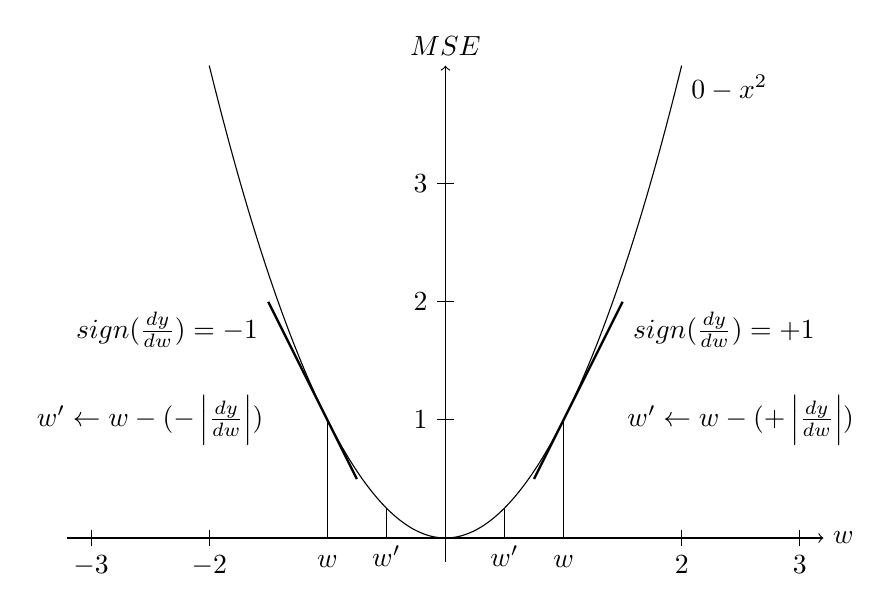
\begin{tikzpicture}[scale=1.5]
      \draw[->] (-3.2,0) -- (3.2,0) node[right] {$w$};
      \draw[->] (0,-0.2) -- (0,4) node[above] {$MSE$};

      \foreach \x/\xtext in {2/2, 3/3}
        \draw[shift={(\x,0)}] (0pt,2pt) -- (0pt,-2pt) node[below] {$\xtext$};
      \foreach \x/\xtext in {-3/-3, -2/-2}
        \draw[shift={(\x,0)}] (0pt,2pt) -- (0pt,-2pt) node[below] {$\xtext$};
      \foreach \y/\ytext in {1/1, 2/2, 3/3}
        \draw[shift={(0,\y)}] (2pt,0pt) -- (-2pt,0pt) node[left] {$\ytext$};

        \draw (-2,4) parabola bend (0,0) (2,4) node[below right] {$\norm{0-x}^2$};
        \draw[-,line width=0.03cm] (0.75,0.5) -- (1.5,2) node[below right] {$sign(\frac{dy}{dw})=+1$};
        \draw[-,line width=0.03cm] (-0.75,0.5) -- (-1.5,2) node[below left] {$sign(\frac{dy}{dw})=-1$};

        \node at (2.5, 1.0) {$w' \leftarrow w - (+\left|\frac{dy}{dw}\right|)$};
        \node at (-2.5, 1.0) {$w' \leftarrow w - (-\left|\frac{dy}{dw}\right|)$};

        \draw[-] (1,1) -- (1,0);
        \draw[-] (-1,1) -- (-1,0);
        \draw[-] (0.5,0.25) -- (0.5,0);
        \draw[-] (-0.5,0.25) -- (-0.5,0);

        \node at (1, -0.2) {$w$};
        \node at (-1, -0.2) {$w$};

        \node at (0.5, -0.15) {$w'$};
        \node at (-0.5, -0.15) {$w'$};
    \end{tikzpicture}
    \caption{Gradient descent for 1-dimensional objective function\label{fig:grad-desc}}
\end{figure}
